\documentclass[]{article}
\usepackage{graphicx}
\usepackage{amsmath}
\usepackage{framed}
%opening
\title{}
\author{}

\voffset=-1.5cm
\oddsidemargin=0.0cm
\textwidth = 470pt
\begin{document}

\maketitle

\begin{abstract}

\end{abstract}
\tableofcontents
\newpage
%------------------------------------------------------ %
\newpage
\section{Control Charts}
{
\large
%\subsection{Control Chart}
%\begin{itemize}
%\item A control chart is a graphical representation of a characteristic of a process, showing plotted values of some statistic, a central line, and one or two control limits. \item It is used to determine whether a process has been operating in statistical control and is an aid to maintaining statistical control.
%\end{itemize}
}
\subsection{Control Charts}
{\large
\begin{itemize}
\item The control chart is a graph used to study how a process changes over time. Data are plotted in time order. A control chart always has a central line for the average, an upper line for the upper control limit and a lower line for the lower control limit. 
\item These lines are determined from historical data. By comparing current data to these lines, you can draw conclusions about whether the process variation is consistent (in control) or is unpredictable (out of control, affected by special causes of variation).

%\item Control charts for variable data are used in pairs. The top chart monitors the average, or the centering of the distribution of data from the process. The bottom chart monitors the range, or the width of the distribution. 
%\item If your data were shots in target practice, the average is where the shots are clustering, and the range is how tightly they are clustered. Control charts for attribute data are used singly.
\end{itemize}
}
\subsection{Control Limits}
{
\large
\begin{itemize}
\item Statistical tables have been developed for various types of distributions that quantify the area under the curve for a given number of standard deviations from the mean (based on the \textbf{\textit{normal distribution}} ).
% These can be used as probability tables to calculate the odds that a given value (measurement) is part of the same group of data used to construct the histogram.
\item Shewhart found that control limits placed at \textit{\textbf{three standard deviations from the mean}} in either direction provide an economical tradeoff between the risk of reacting to a false signal and the risk of not reacting to a true signal - regardless the shape of the underlying process distribution.
\item If the process has a normal distribution, 99.7\% of the population is captured by the curve at three standard deviations from the mean. Stated another way, there is only a 100-99.7\%, or 0.3\% chance of finding a value beyond 3 standard deviations. Therefore, a measurement value beyond 3 standard deviations indicates that the process has either shifted or become unstable (more variability).
\end{itemize}
}
\newpage
\begin{figure}[h!]
\centering
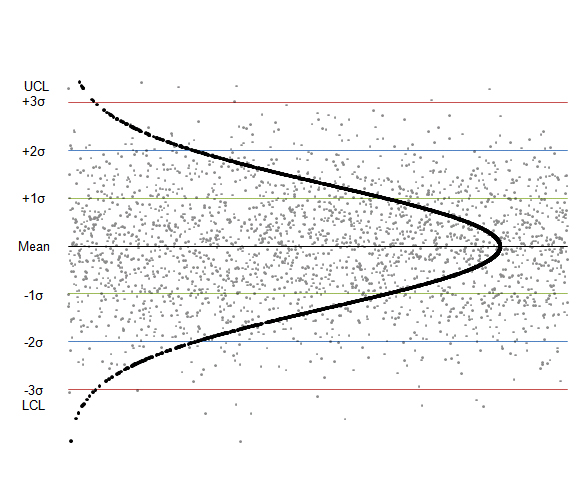
\includegraphics[width=0.8
\linewidth]{./ControlChart}

\label{fig:ControlChart}
\end{figure}
\newpage
\section{Ten R Packages that every Data Scientist Should know}

\subsection{10 R packages I wish I knew about earlier}
\begin{itemize}
\item \textit{Following material written by Drew Conway, and was published on the Yhat blog Feb 2013} \item \textit{http://blog.yhathq.com/posts/10-R-packages-I-wish-I-knew-about-earlier.html}
\end{itemize}

{\large
\begin{itemize}
\item \textbf{qcc} is a library for statistical quality control. Back in the 1950s, the now defunct Western Electric Company was looking for a better way to detect problems with telephone and eletrical lines.

\subitem \textit{\textbf{Remark}: We will discuss these rules shortly}

 \item They came up with a set of rules to help them identify problematic lines. The rules look at the historical mean of a series of datapoints and based on the standard deviation, the rules help judge whether a new set of points is experiencing a mean shift.

\item The classic example is monitoring a machine that produces lug nuts. \\ Let's say the machine is supposed to produce 2.5 inch long lug nuts. We measure a series of lug nuts: 2.48, 2.47, 2.51, 2.52, 2.54, 2.42, 2.52, 2.58, 2.51. \item  Is the machine broken? Well it's hard to tell, but the \textit{Western Electric} Rules can help.

\item While you might not be monitoring telephone lines, qcc can help you monitor transaction volumes, visitors or logins on your website, database operations, and lots of other processes.
\end{itemize}}
\newpage
\subsubsection{Other Remarks}
{\large
\begin{itemize}
\item Quality Control and quality assurance are important functions in most businesses from manufacturing to software development. 
\item For most, this means that one or more people are meticulously inspecting what's coming out of the factory, looking for imperfections and validating that requirements for products and services produced are satisfied. \item Often times QC and QA are performed manually by a select few specialists, and determining suitable quality can be extremely complex and error-prone.
\end{itemize}}
\newpage
{
\large
\begin{framed}
\begin{verbatim}
# install.package(qcc)
library(qcc)
 
# series of value w/ mean of 10 with a little random noise added in
x <- rep(10, 100) + rnorm(100)

# a test series w/ a mean of 11
new.x <- rep(11, 15) + rnorm(15)

# qcc will flag the new points
qcc(x, newdata=new.x, type="xbar.one")
\end{verbatim}
\end{framed}
}
% END OF PAGE 1
% GOOD SO FAR 



\begin{figure}[h!]
\centering
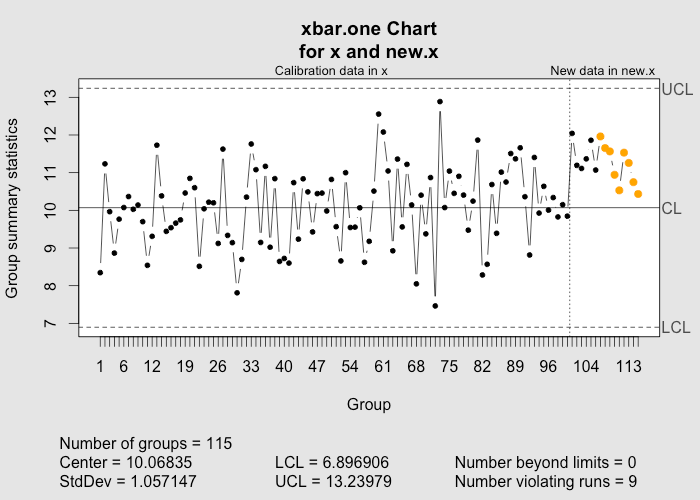
\includegraphics[width=0.9\linewidth]{./qcc-yhatexample}
\caption{}
\label{fig:qcc-yhatexample}
\end{figure}
\bigskip
\newpage
%-------------------------------------------- %
\begin{figure}[h!]
\centering
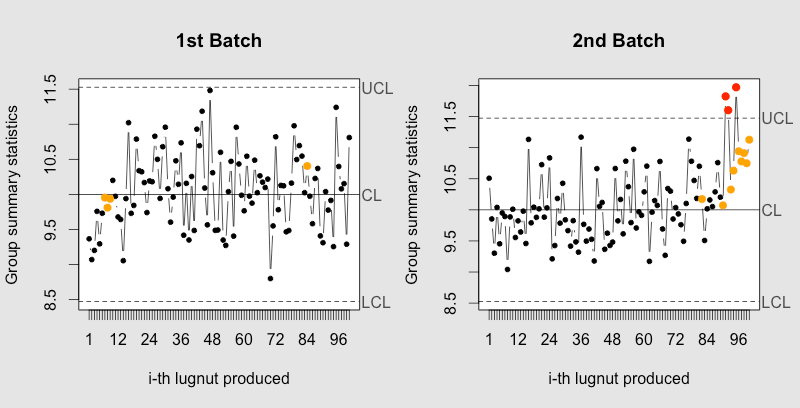
\includegraphics[width=0.90\linewidth]{./qcc_lugnuts1}

\label{fig:qcc_lugnuts1}
\end{figure}
\begin{framed}
\begin{verbatim}
library(qcc)
#make 2 plots in 1 figure
par(mfrow=c(1,2))
 
#points have base value of 10 w/ normally distributed error
lugnuts <- rep(10, 100) + rnorm(100, mean=0, sd=0.5)
qcc(lugnuts, type="xbar.one", center=10, add.stats=FALSE,
    title="1st Batch", 
    xlab="i-th lugnut produced")
\end{verbatim}
\end{framed} 
{
\large
\textbf{Second Batch }
\begin{itemize}
\item First 90 points have mean value of 10 with normally distributed error,
\item Last 10 points have mean value of 11 with normally distributed error
\end{itemize}
}
\begin{framed}
\begin{verbatim}
lugnuts <- c(rep(10, 90), rep(11, 10)) + rnorm(100, mean=0, sd=0.5)
qcc(lugnuts, type="xbar.one", center=10, add.stats=FALSE,
    title="2nd Batch", 
    xlab="i-th lugnut produced")
 
\end{verbatim}
\end{framed}
\newpage 

\begin{verbatim}
> set.seed(1234)
> lugnuts <- rep(10, 100) + rnorm(100, mean=0, sd=0.5)
> summary(lugnuts)
   Min. 1st Qu.  Median    Mean 3rd Qu.    Max. 
  8.827   9.552   9.808   9.922  10.240  11.270 
> length(lugnuts)
[1] 100
> newLugnuts <- rep(11, 10) + rnorm(10, mean=0, sd=0.5)
> summary(newLugnuts)
   Min. 1st Qu.  Median    Mean 3rd Qu.    Max. 
  10.55   10.75   11.00   10.92   11.08   11.21 
> length(newLugnuts)
[1] 10
\end{verbatim}

\begin{framed}
\begin{verbatim}
qcc1 <- qcc(lugnuts, type="xbar.one", center=10, add.stats=TRUE,
    title="1st Batch of 100", 
    xlab="i-th lugnut produced")



qcc2 <- qcc(lugnuts, newdata=newLugnuts,
    type="xbar.one", center=10, 
    add.stats=TRUE, title="All Lugnuts", 
    xlab="i-th lugnut produced")

mode(qcc1)
class(qcc1)
names(qcc1)
\end{verbatim}
\end{framed}

\begin{verbatim}
> mode(qcc1)
[1] "list"
> class(qcc1)
[1] "qcc"
> names(qcc1)
 [1] "call"       "type"       "data.name"  "data"       "statistics"
 [6] "sizes"      "center"     "std.dev"    "nsigmas"    "limits"    
[11] "violations"
> qcc1$violations
$beyond.limits
integer(0)

$violating.runs
 [1] 13 38 39 40 48 49 50 51 52 53 54 55
\end{verbatim}

\newpage
\begin{figure}[h!]
\centering
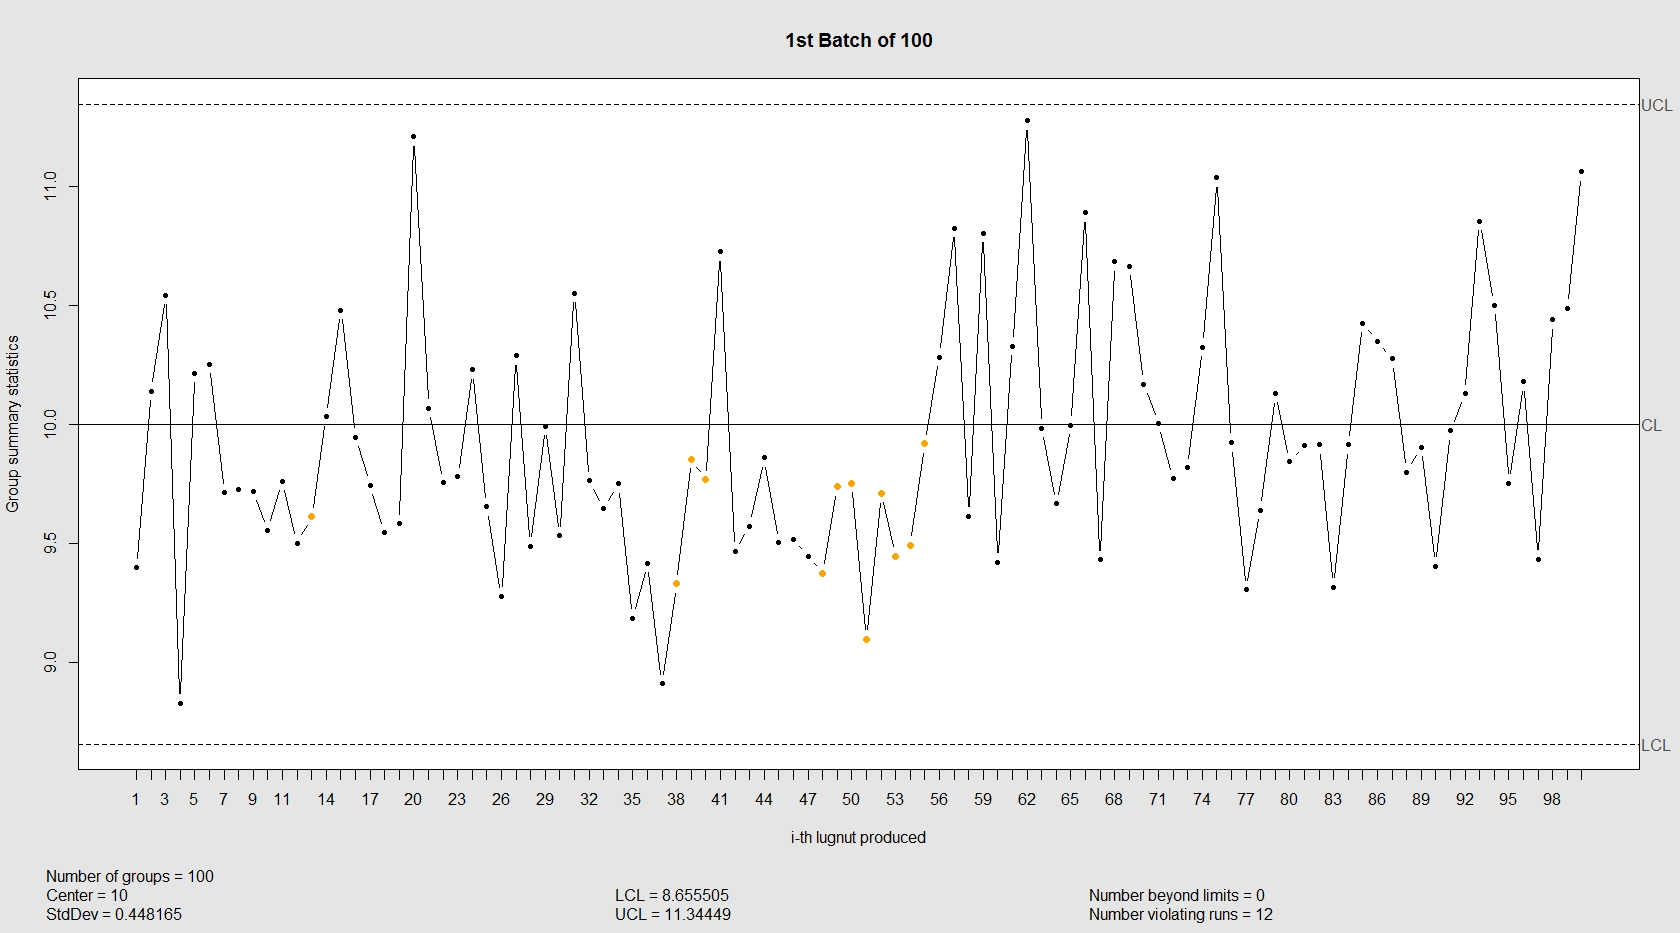
\includegraphics[width=0.8\linewidth]{./lugnuts1}
\caption{}
\label{fig:lugnuts1}
\end{figure}
\begin{figure}[h!]
\centering
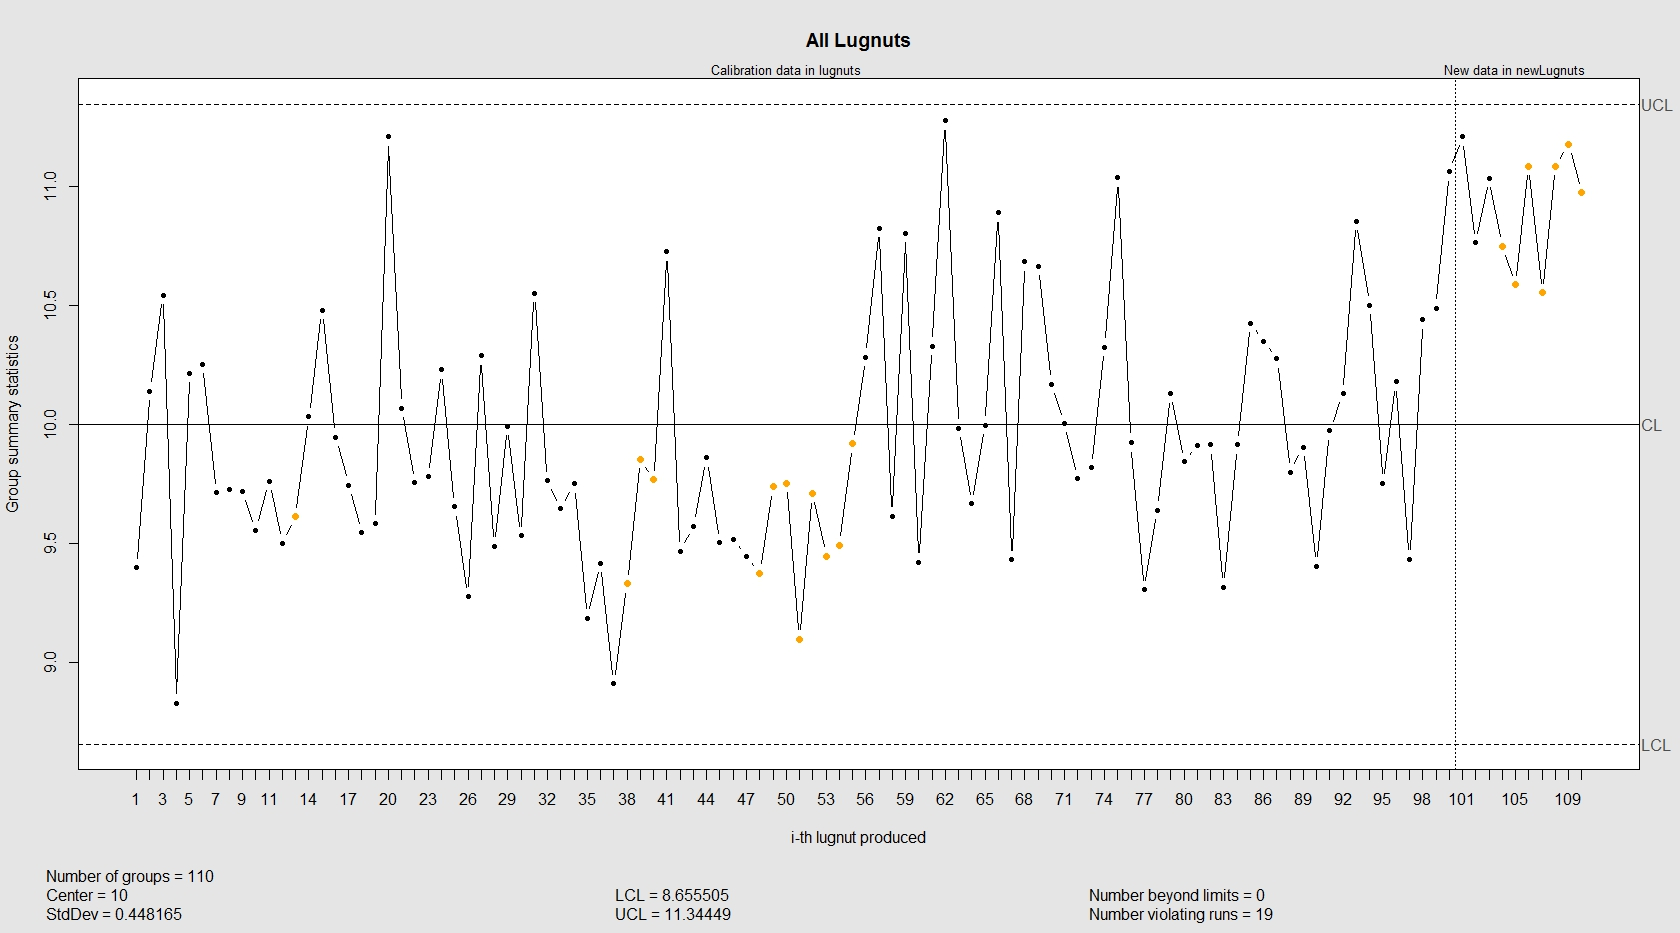
\includegraphics[width=0.8\linewidth]{./lugnuts2}
\caption{}
\label{fig:lugnuts2}
\end{figure}
\newpage
\subsection{Using the \texttt{summary} command}
\begin{framed}
\begin{verbatim}
Call:
qcc(data = lugnuts, type = "xbar.one", center = 10, add.stats = TRUE,     
title = "1st Batch of 100", xlab = "i-th lugnut produced")

xbar.one chart for lugnuts 

Summary of group statistics:
   Min. 1st Qu.  Median    Mean 3rd Qu.    Max. 
  8.827   9.552   9.808   9.922  10.240  11.270 

Group sample size:  1
Number of groups:  100
Center of group statistics:  10
Standard deviation:  0.448165 

Control limits:
      LCL      UCL
 8.655505 11.34449
\end{verbatim}
\end{framed}
\begin{framed}
\begin{verbatim}
Call:
qcc(data = lugnuts, type = "xbar.one", center = 10, newdata = newLugnuts,     
add.stats = TRUE, title = "All Lugnuts", xlab = "i-th lugnut produced")

xbar.one chart for lugnuts 
.....

Summary of group statistics in newLugnuts:
   Min. 1st Qu.  Median    Mean 3rd Qu.    Max. 
  10.55   10.75   11.00   10.92   11.08   11.21 

Group sample size:  1
Number of groups:  10 

Control limits:
      LCL      UCL
 8.655505 11.34449

\end{verbatim}
\end{framed}
\newpage

\subsubsection{Example used by Drew Conway}
\begin{figure}[h!]
\centering
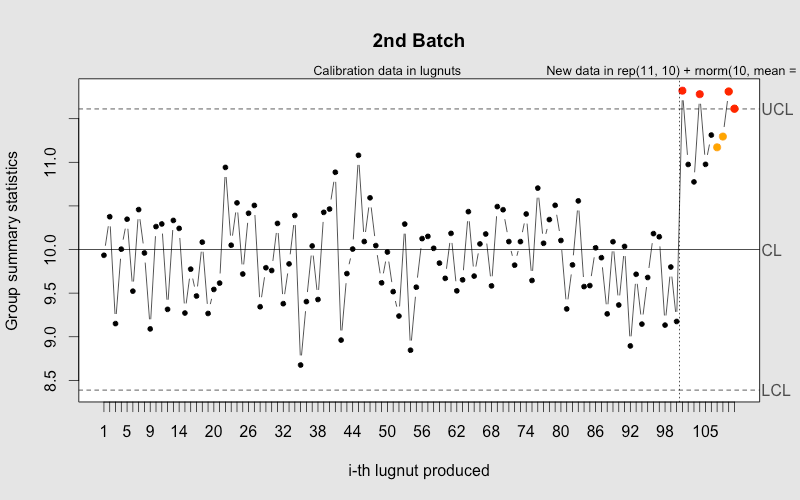
\includegraphics[width=0.7\linewidth]{./qcc_holdout2}
\caption{}
\label{fig:qcc_holdout2}
\end{figure}
\begin{framed}
\begin{verbatim} 

lugnuts <- rep(10, 100) + rnorm(100, mean=0, sd=0.5)
qcc(lugnuts, newdata=rep(11, 10) + rnorm(10, mean=0, sd=0.5),
    type="xbar.one", center=10, 
    add.stats=FALSE, title="2nd Batch", 
    xlab="i-th lugnut produced")
\end{verbatim}
\end{framed}

\subsubsection{Remarks}
{\large
\begin{itemize}
\item \texttt{newdata}
\item \texttt{add.stats }
\end{itemize}}
\newpage





\subsection{Using R}
{
\large
Advantages of using R statistical program along with the \textbf{qcc} package:
\begin{itemize}
\item There are several packages for interfacing with databases, RODBC being a common and useful one on MS windows.
\item Allows of automation: you can program a regular event loop to check for new data and run a new set of charts and notifications if there is new data.
\item The \textbf{mail} and \textbf{sendmailR} packages were designed to automatically send e-mails with regular reports and warning messages.
\item It produces the standard SPC charts, these can go to the screen or a file to be sent out.
\item Bespokes tests can be program for out of control signals
\item Full programming language with common (and uncommon) statistics so you can pre-proccess you data in many ways to reduce dimension.
\item You can have multiple instances running on multiple or a single computer, each processing for a single department, or you can combine it all into one script to run for all the departments.
\end{itemize}
}
%------------------------------------------------------ % 
\newpage
\section{What is Statistical Process Control}
{
\large
\begin{itemize}
\item The concepts of Statistical Process Control (SPC) were initially developed by Dr. Walter Shewhart of Bell Laboratories in the 1920's, and were expanded upon by Dr. W. Edwards Deming, who introduced SPC to Japanese industry after WWII.
\item After early successful adoption by Japanese firms, Statistical Process Control has now been incorporated by organizations around the world as a primary tool to improve product quality by reducing process variation.
\item Dr. Shewhart identified two sources of process variation: 
\begin{description}
\item[Chance variation] that is inherent in process, and stable over time, 
\item[Assignable variation], or Uncontrolled variation, which is unstable over time - the result of specific events outside the system.
\end{description}
 
\item Dr. Deming relabeled chance variation as \textbf{Common Cause} variation, and assignable variation as \textbf{Special Cause} variation.
\item Based on experience with many types of process data, and supported by the laws of statistics and probability, Dr. Shewhart devised control charts used to plot data over time and identify both Common Cause variation and Special Cause variation.
\end{itemize}
}
%------------------------------------------------------ % 
%\newpage
%\subsection{Deming's Seminars in Japan}
%
%This article attempts to clarify the role played by W. Edwards Deming at the beginning of the modern Japanese quality control movement by summarizing and analyzing the actual content of the series of quality control lectures he gave in Japan during the summer of 1950. The primary source documents are the published lecture transcripts that Deming considered authentic.Analysis of the transcripts shows that Deming spent most of the eight-day lecture series discussing statistical process control. 
%
%
%However, he opened the lectures with extended remarks that contain a core of the philosophy for which he later became famous. Yet, significant elements of what is now known as the Deming method or Deming philosophy did not appear in the lecture series. Deming included in the lectures an extended discussion of sampling inspection that revealed his ambivalence to the subject. The transcripts show that Deming introduced to the Japanese a product design cycle of Shewhart that is distinct from the management process that the Japanese later came to call the plan-do-check-act cycle.
%------------------------------------------------------ % 

\subsection{Some Remarks on Multivariate Techniques}
%MSQC book
{
\large

\begin{itemize}
\item Nowadays, the intensive use of an automatic data acquisition systems and the use of
on-line computers for process monitoring have led to an increased occurrence of
industrial processes with two or more correlated quality characteristics, in which
the statistical process control and the capability analysis should be performed using
multivariate methodologies. \textit{(Edgar Santos-Fernandez)}
\end{itemize}
}


\newpage
\subsection{7 Basic Tools of Quality }
{\large
These are 7 QC tools also known as Ishikawas \textbf{7QC} tools
\begin{description}
\item[Cause-and-effect diagram]: Identifies many possible causes for an effect or problem and sorts ideas into useful categories.
(also called \textit{Ishikawa} or\textit{ fishbone chart})

\item[Check sheet]: A structured, prepared form for collecting and analyzing data; a generic tool that can be adapted for a wide variety of purposes.

\item[Control charts]: Graphs used to study how a process changes over time.

\item[Histogram]: The most commonly used graph for showing frequency distributions, or how often each different value in a set of data occurs.

\item[Pareto chart]: Shows on a bar graph which factors are more significant.

\item[Scatter diagram]: Graphs pairs of numerical data, one variable on each axis, to look for a relationship.

\item[Stratification]: A technique that separates data gathered from a variety of sources so that patterns can be seen (some lists replace “stratification” with “flowchart” or “run chart”).
\end{description}
For the sake of brevity, we will only look at a couple of these.
}


\newpage


%------------------------------------------------------ % 
\newpage
\subsection{Testing for Normality}
%MSQC
{
\large
\textbf{Graphical Methods}
\begin{itemize}
\item Histograms
\item Normal Probability Plots
\end{itemize}

\noindent\textbf{Hypothesis Tests for Univariate Data}
\begin{itemize}
\item Shapiro-Wilk Test (inbuilt with \texttt{R})
\item D'Agostino Test (MSQC package)
\end{itemize}
\bigskip

\noindent\textbf{Hypothesis Tests for Multivariate Data}
\begin{itemize}
\item Mardia Test (MSQC package)
\item Henze and Zirkler (MSQC package)
\item Royston Test (MSQC package)
\end{itemize}


}
\newpage
\subsubsection{The bimetal data set (MSQC package)}
\begin{framed}
\begin{verbatim}
> tail(bimetal1)
      deflection curvature resistivity Hardness low side Hardness high side
[23,]      20.76     39.98       14.98             22.29              26.03
[24,]      21.00     40.11       15.17             22.04              25.99
[25,]      20.57     39.73       14.35             22.02              25.80
[26,]      20.78     39.83       15.27             21.60              25.89
[27,]      20.96     40.03       15.26             21.98              25.94
[28,]      21.14     39.93       14.98             21.84              25.98

\end{verbatim}
\end{framed}

\newpage
\begin{figure}[h!]
\centering
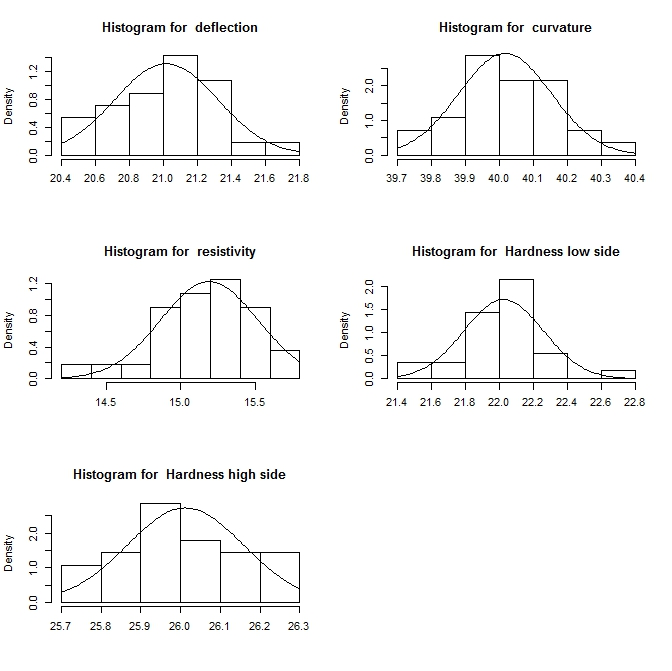
\includegraphics[width=0.9\linewidth]{./MSQC-bimetal1hist}
\caption{}
\label{fig:MSQC-bimetal1hist}
\end{figure}
\newpage
\begin{figure}[h!]
\centering
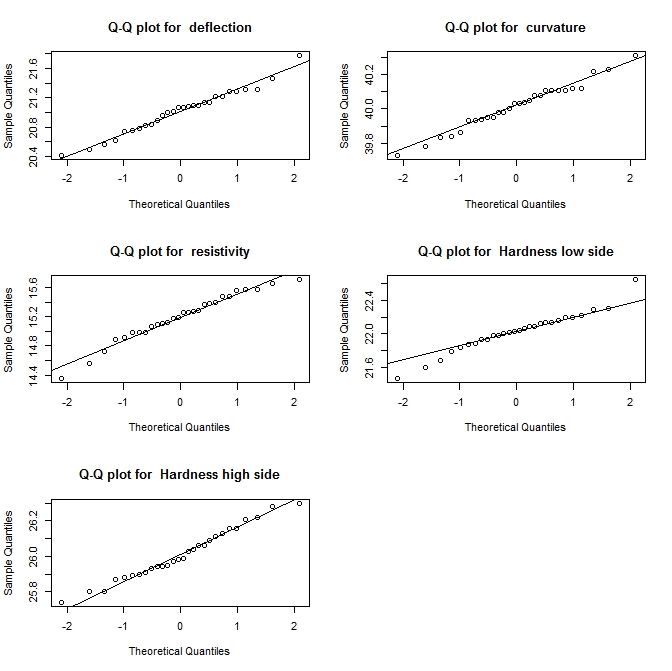
\includegraphics[width=0.9\linewidth]{./MSQC-bimetal1qq}
\caption{}
\label{fig:MSQC-bimetal1qq}
\end{figure}
\newpage
\subsubsection{D'Agostino Test (MSQC Pacakge)}
\begin{itemize}
\item Using the bimetal1 data set in MSQC package
\end{itemize}
\begin{framed}
\begin{verbatim}
> for (i in 1 : 5){
+  DAGOSTINO(bimetal1[,i])
+  }
D'Agostino Test
    Skewness
      Skewness coefficient: 0.0831225 
      Statistics: 0.2117358 
      p-value: 0.8323131 
    Kurtosis
      The kurtosis coefficient: 3.0422 
      Statistics: 0.591983 
      p-value: 0.553862 
    Omnibus Test
      Chi-squared: 0.3952759 
      Degree of freedom: 2
      p-value: 0.8206669 
....
....
D'Agostino Test
    Skewness
      Skewness coefficient: -0.04173762 
      Statistics: -0.1063873 
      p-value: 0.9152751 
    Kurtosis
      The kurtosis coefficient: 4.162062 
      Statistics: 1.675258 
      p-value: 0.09388364 
    Omnibus Test
      Chi-squared: 2.817807 
      Degree of freedom: 2
      p-value: 0.2444111 
\end{verbatim}
\end{framed}
\newpage
\subsubsection{Some Multivariate (MSQC Pacakge)}
\begin{framed}
\begin{verbatim}
> MardiaTest(bimetal1)
$skewness
[1] 6.982112

$p.value
[1] 0.585327

$kurtosis
[1] 33.77373

$p.value
[1] 0.3490892

> 
>
>
> HZ.test(bimetal1)
[1] 0.6068650 0.7709586
> 
> 
> Royston.test(bimetal1)
test.statistic        p.value 
     1.1814742      0.9364221 
\end{verbatim}
\end{framed}




\subsubsection{Box Cox Transformation}
\begin{itemize}
\item The Box-Cox transforms nonnormally distributed data to a set of  data that has approximately normal distribution. 
\end{itemize}
\newpage
\subsection{Multivariate Normal}
{\large
\begin{itemize}
\item The multivariate normal distribution or multivariate Gaussian distribution, is a generalization of the one-dimensional (univariate) normal distribution to higher dimensions.\item One possible definition is that a random vector is said to be k-variate normally distributed if every linear combination of its k components has a univariate normal distribution. 
%\item However, its importance derives mainly from the multivariate central limit theorem.
\item The multivariate normal distribution is often used to describe, at least approximately, any set of (possibly) correlated real-valued random variables each of which clusters around a mean value.
\end{itemize}
}
\begin{figure}[h!]
\centering
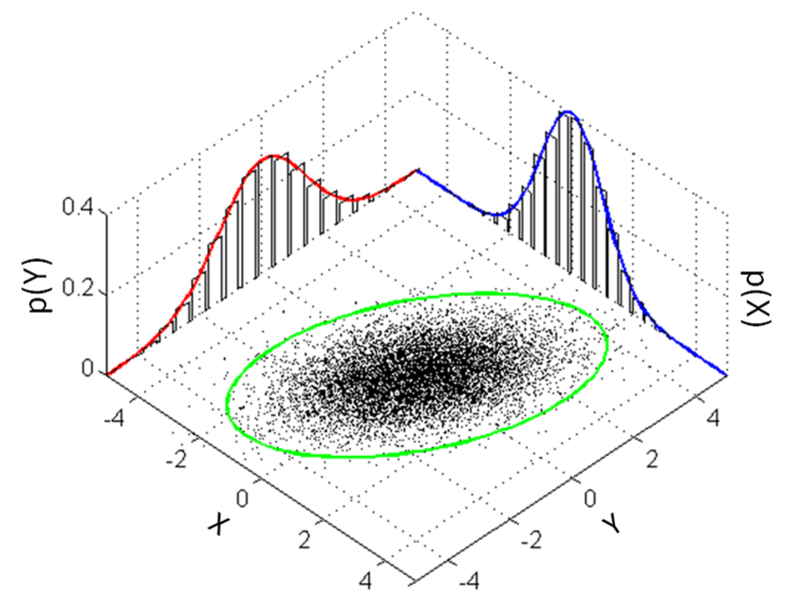
\includegraphics[width=0.8\linewidth]{./793px-MultivariateNormal}
\caption{}
\label{fig:793px-MultivariateNormal}
\end{figure}

\newpage
%------------------------------------------------------ % 

\section{Nelson Rules for Interpreting Control Charts}
{\large
\begin{itemize}
\item The eight tests used in statistical process control were developed by Lloyd S. Nelson, a process control expert. They are
based on his determination that the identified patterns are very unlikely to occur in stable processes.

\item Thus
the existence of any of these patterns in an $\bar{X}$ chart indicates that the process may be unstable, and that one or
more assignable causes may exist. 

\item The table on the next page contains examples of test failure for each of the eight tests,
with a description for each graph as to what is required for the illustrated test failure.

\item In practice, tests 1,2 and 7 are considered the three most useful.
\end{itemize}
}
{
\large
\subsection{Descriptions of Tests}
\begin{description}
\item[Test 1 - 3 sigma rule] Identifies points outside of the control limits\\
Test 1 identifies points that are more standard deviations from the center line. Test 1 is
universally recognized as necessary for detecting out-of-control situations. It has a
false alarm rate of only 0.27\%.

\item[Test 2] Identifies shifts in the means \\
Test 2 signals when 9 points in a row fall on the same side of the center line.  The use of Test 2
significantly increases the sensitivity of the chart to detect small shifts in the mean.

When test 1 and test 2 are used together, significantly fewer subgroups are needed
to detect a small shift in the mean than are needed when test 1 is used alone.
Therefore, adding test 2 helps to detect common out-of-control situations and
increases sensitivity enough to warrant a slight increase in the false alarm rate.
\end{description}
}
\newpage
\begin{figure}[h!]
  % 
  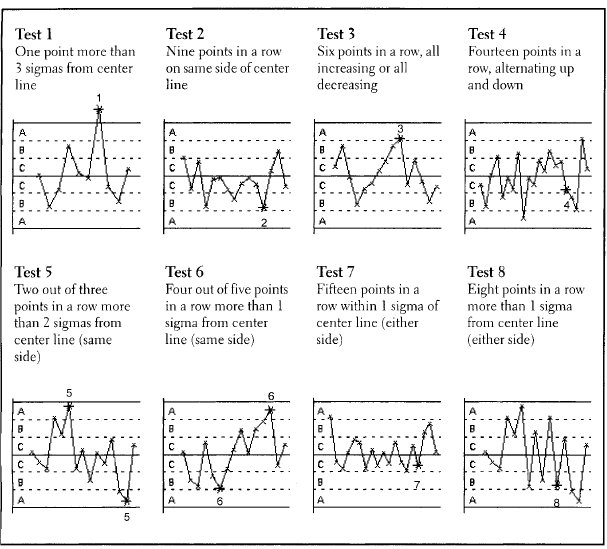
\includegraphics[scale=0.90]{WECOtests}\\
  %\caption{WECO Tests}\label{WECO}
\end{figure}

\newpage

\newpage
{
\large
\begin{description}
\item[Test 3] $k$ points in a row, all increasing or all decreasing\\
Test 3 is designed to detect drifts in the process mean.\\
However, when test 3 is used in addition to test 1 and test 2, it does not
significantly increase the sensitivity of the chart to detect drifts in the process
mean.


\item[Test 4] $k$ points in a row, alternating up and down\\
Although this pattern can occur in practice, it is recommended to search for any
unusual trends or patterns rather than test for one specific pattern.
\item[Test 5] $k$ out of k=1 points $> 2$ standard deviations from center line\\
This test is not quite as informative because it did not
uniquely identify special cause situations that are common in practice.
\item[Test 6] $k$ out of k+1 points $> 1$ standard deviation from the center line\\
This test is not quite as informative because it did not
uniquely identify special cause situations that are common in practice.

\item[Test 7] Identifies control limits that are too wide\\
Test 7 signals when 12 or 15 points in a row fall within 1 standard deviation of the
center line.\\ Test 7 is used only for the $\bar{X}$ chart when the control limits are
estimated from the data. When this test fails, the cause is usually a systemic source
of variation (stratification) within a subgroup, which is often the result of not 
forming rational subgroups. 
\item[Test 8] $k$ points in a row $> 1$ standard deviation from center line (either
side)\\
This test is not quite as informative because it did not
uniquely identify special cause situations that are common in practice.
\end{description}
}
\newpage
\section{Multivariate Control Charts}
{\large
%MSQC book Part 2
With the enhancements in data acquisition systems it is usual to deal with processes
with more than one correlated quality characteristic to be monitored. A common
practice is to control the stability of the process using univariate control charts. This
practice increases the probability of false alarm of special cause of variation.
Therefore, the analysis should be performed through a multivariate approach;
that is, the variables must be analyzed together, not independently.
In this chapter we present the multivariate normal distribution, the data structure
of the multivariate problems dealt in this book, the mult.chart function that allows
the computation in R, and the most used multivariate control charts:
}
\begin{itemize}
\item The control ellipsoid or w2 control chart
\item The T2 or Hotelling chart
\item The Multivariate Exponentially Weighted Moving Average (MEWMA) chart
\item The Multivariate Cumulative Sum (MCUSUM) chart
\item The chart based on Principal Components Analysis (PCA)
\end{itemize} 

 
 \begin{figure}
\centering
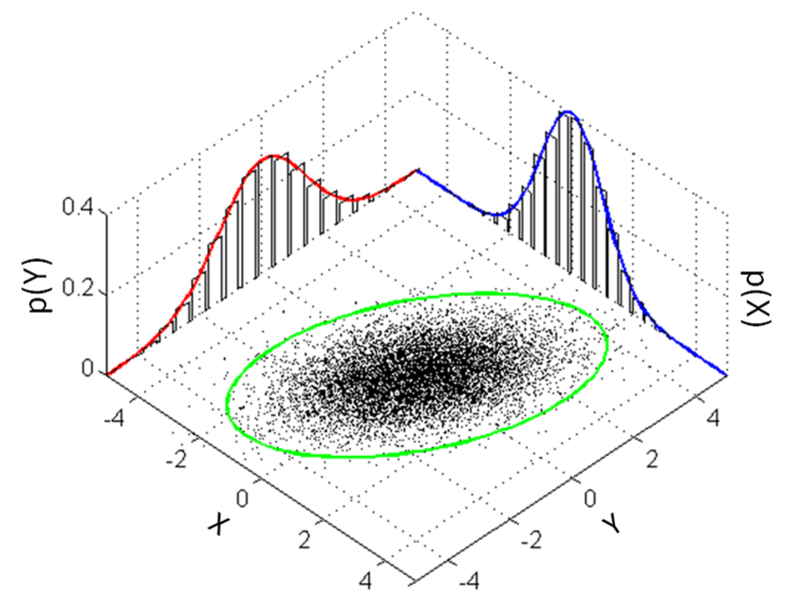
\includegraphics[width=0.7\linewidth]{./793px-MultivariateNormal}
\caption{}
\label{fig:793px-MultivariateNormal}
\end{figure}

\subsection{Confidence Region}
a confidence region is a multi-dimensional generalization of a confidence interval. It is a set of points in an n-dimensional space, often represented as an ellipsoid around a point which is an estimated solution to a problem, although other shapes can occur.

The confidence region is calculated in such a way that if a set of measurements were repeated many times and a confidence region calculated in the same way on each set of measurements, then a certain percentage of the time, on average, (e.g. 95%) the confidence region would include the point representing the "true" values of the set of variables being estimated. However, unless certain assumptions about prior probabilities are made, it does not mean, when one confidence region has been calculated, that there is a 95% probability that the "true" values lie inside the region, since we do not assume any particular probability distribution of the "true" values and we may or may not have other information about where they are likely to lie.
\newpage

\section{The \textbf{qcc} R package - The 7QC tools revisited}
The qcc package

%Yhat Blog

So we've come up with a good framework for our problem, now what?. Enter the qcc package in R. This magical little library was built by Luca Scrucca for nothing but statistical quality control. It's extremely easy to use. You provide it with data and it tells you which points are considered to be outliers based on the Shewart Rules. It even color codes them based on how irregular each point is. In the example below you can see that for the last 10 points of the 2nd dataset I shifted the mean of the data from 10 to 11.
% %

Even though it's an old topic, statistical quality control is still highly relevant. While you might not be working at a lug nut factory, you probably have lots of jobs, processes, logs, or databse metric that you could monitor using control charts.

\textbf{Quality Control Charts}

\begin{itemize}
\item Shewhart quality control charts for continuous, attribute and count data.
\item Cusum and EWMA charts. 
\item Operating characteristic curves.
\item Process capability analysis. 
\item Pareto chart and cause-and-effect chart. 
\item Multivariate control charts.
\end{itemize}



\subsection{Cause and Effect Diagrams}
The cause and effect diagram is also known as ``Ishikawa diagram", and has been widely used in
Quality Management. It is one of the Seven Basic Tools of Quality.
\begin{framed}
\begin{verbatim}
effect <- "Flight Time"
causes.gr <- c("Operator", "Environment", "Tools", "Design",
"Raw.Material", "Measure.Tool")
causes <- vector(mode = "list", length = length(causes.gr))
causes[1] <- list(c("operator #1", "operator #2", "operator #3"))
causes[2] <- list(c("height", "cleaning"))
causes[3] <- list(c("scissors", "tape"))
causes[4] <- list(c("rotor.length", "rotor.width2", "paperclip"))
causes[5] <- list(c("thickness", "marks"))
causes[6] <- list(c("calibrate", "model"))
ss.ceDiag(effect, causes.gr, causes, sub = "Paper Helicopter Project")
\end{verbatim}
\end{framed}
\begin{figure}[h!]
\centering
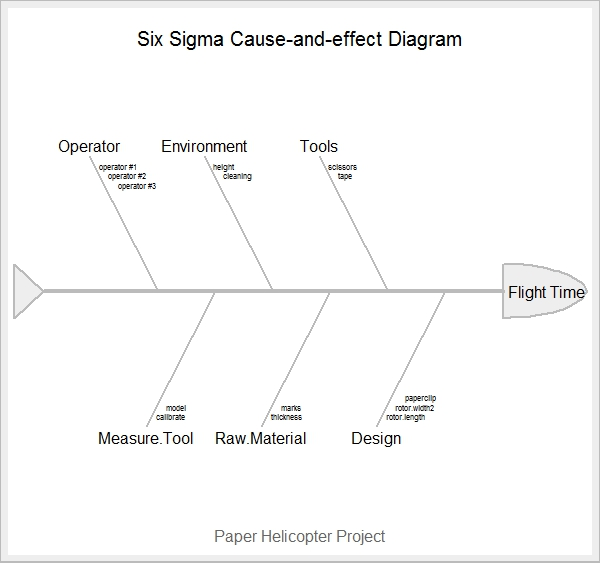
\includegraphics[width=0.7\linewidth]{./Rplot03}
\caption{}
\label{fig:Rplot03}
\end{figure}
\begin{framed}
\begin{verbatim}
cause.and.effect(cause=list(
  Measurements=c("Micrometers", "Microscopes", "Inspectors"),
  Materials=c("Alloys", "Lubricants", "Suppliers"),
  Personnel=c("Shofts", "Supervisors", "Training", "Operators"),
  Environment=c("Condensation", "Moisture"),
  Methods=c("Brake", "Engager", "Angle"),
  Machines=c("Speed", "Lathes", "Bits", "Sockets")),
effect="Surface Flaws")
\end{verbatim}
\end{framed}
\begin{figure}[h!]
\centering
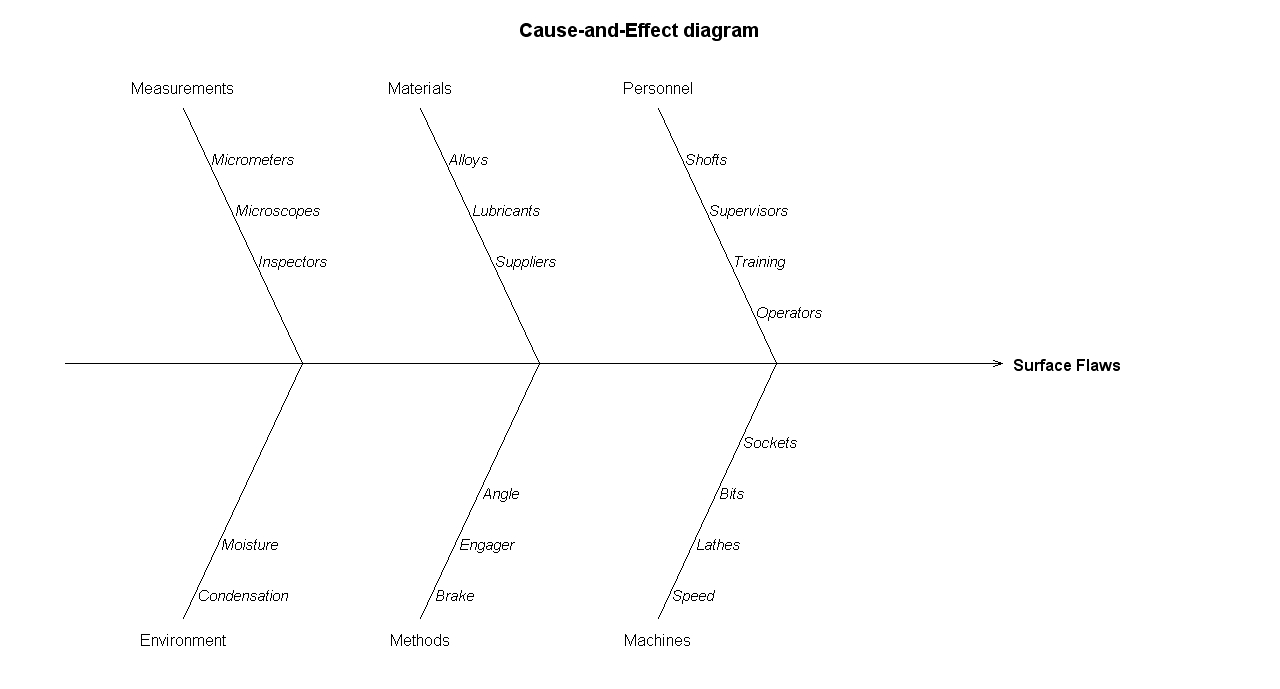
\includegraphics[width=0.7\linewidth]{./qccfishbone}
\caption{}
\label{fig:qccfishbone}
\end{figure}

\newpage
\subsection{Pareto Chart Analysis.}
 Quality problems are rarely spread evenly across the different aspects of the production process or different plants. Rather, a few "bad apples" often account for the majority of problems. This principle has come to be known as the Pareto principle, which basically states that quality losses are mal-distributed in such a way that a small percentage of possible causes are responsible for the majority of the quality problems. For example, a relatively small number of "dirty" cars are probably responsible for the majority of air pollution; the majority of losses in most companies result from the failure of only one or two products. To illustrate the "bad apples", one plots the Pareto chart,
\newpage
\subsection{Pareto Analysis (Implementation with qcc package)}
\begin{framed}
\begin{verbatim}
defect <- c(80, 27, 66, 94, 33)

names(defect) <- c("price code", "schedule date", 
 "supplier code", "contact num.", "part num.")

# 1
pareto.chart(defect, ylab = "Error frequency")

#2
pareto.chart(defect, ylab = "Error frequency", xlab = "Error causes", las=1)

#3
pareto.chart(defect, ylab = "Error frequency", col=rainbow(length(defect)))

#4
pareto.chart(defect, cumperc = seq(0, 100, by = 5), 
    ylab2 = "A finer tickmarks grid")

\end{verbatim}
\end{framed}
\textbf{Output to accompany graphs}
\begin{verbatim}
Pareto chart analysis for defect
                Frequency Cum.Freq. Percentage Cum.Percent.
  contact num.         94        94   31.33333     31.33333
  price code           80       174   26.66667     58.00000
  supplier code        66       240   22.00000     80.00000
  part num.            33       273   11.00000     91.00000
  schedule date        27       300    9.00000    100.00000
\end{verbatim}
%------------------------------------------- %
\newpage

\begin{figure}[h!]
\centering
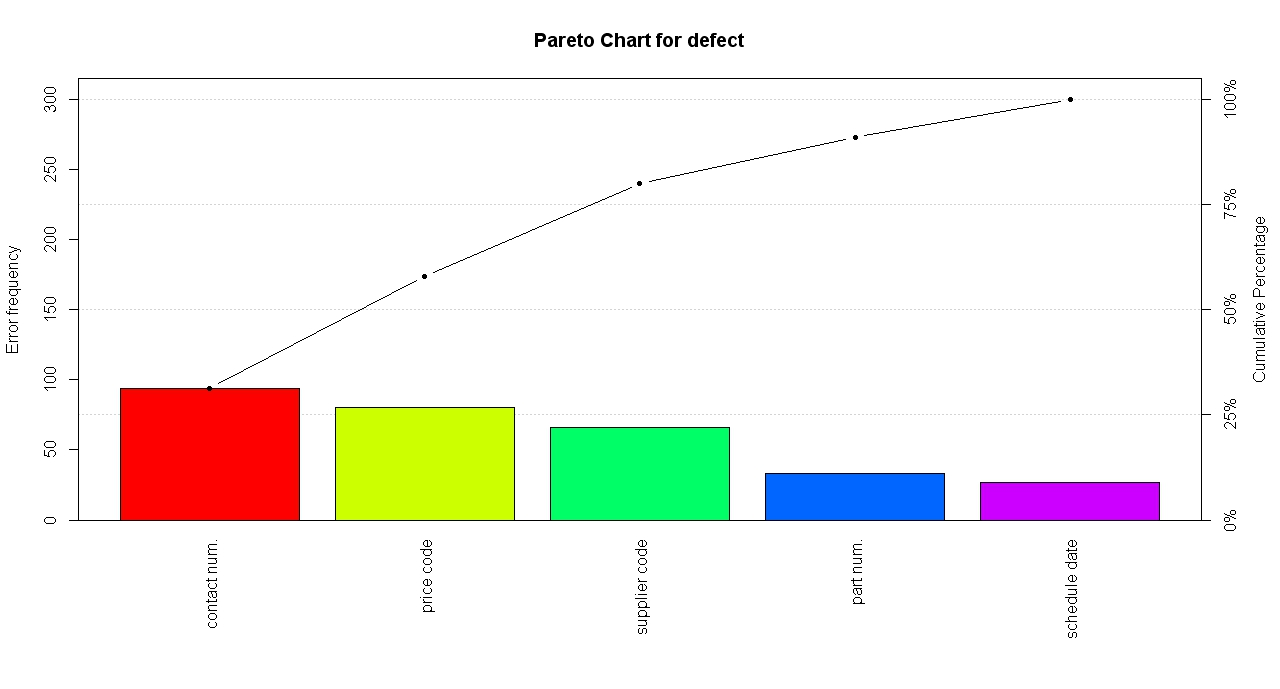
\includegraphics[width=0.8\linewidth]{./Pareto3}
\caption{Third Implementation}
\label{fig:Pareto3}
\end{figure}

\begin{figure}[h!]
\centering
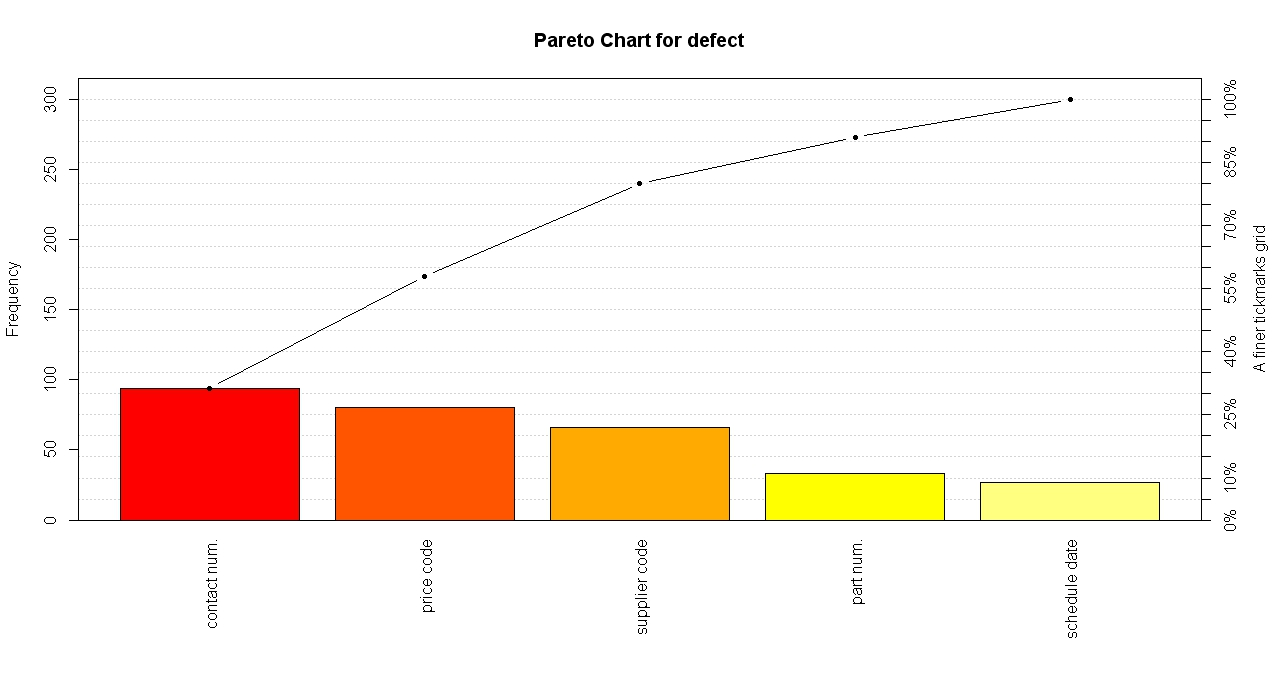
\includegraphics[width=0.8\linewidth]{./Pareto5}
\caption{Fourth Implementation}
\label{fig:Pareto5}
\end{figure}

\section{More on Control Charts}

\newpage
\subsection{Control Chart Selection}
\begin{itemize}
\item Correct control chart selection is a critical part of creating a control chart. If the wrong control chart is selected, the control limits will not be correct for the data. 
\item The type of control chart required is determined by the type of data to be plotted and the format in which it is collected. \item Data collected is either in variables or attributes format, and the amount of data contained in each sample (subgroup) collected is specified.

\item \textbf{Variables data} is defined as a measurement such as height, weight, time, or length. Monetary values are also variables data. 
\begin{itemize}
\item[$\ast$] Generally, a measuring device such as a weighing scale, vernier, or clock produces this data. \item[$\ast$] Another characteristic of variables data is that it can contain decimal places e.g. 3.4, 8.2.
\end{itemize}

\item \textbf{Attributes data} is defined as a count such as the number of employees, the number of errors, the number of defective products, or the number of phone calls. A standard is set, and then an assessment is made to establish if the standard has been met. 
\begin{itemize}
\item[$\ast$] The number of times the standard is either met or not is the count. Attributes data never contains decimal places when it is collected, it is always whole numbers, e.g. 2, 15.
\end{itemize}
\end{itemize}

%------------------------------------------------------------- %
\newpage

\subsection{Attribute Control Charts}

\begin{itemize}
\item The Shewhart control chart plots quality characteristics that can be measured and expressed numerically. We measure weight, height, position, thickness, etc. If we cannot represent a particular quality characteristic numerically, or if it is impractical to do so, we then often resort to using a quality characteristic to sort or classify an item that is inspected into one of two "buckets".
\item  An example of a common quality characteristic classification would be designating units as "conforming units" or "nonconforming units". 
\item Another quality characteristic criteria would be sorting units into "non defective" and "defective" categories. Quality characteristics of that type are called \textit{\textbf{attributes}}.

\item \textit{Note that there is a difference between "nonconforming to an engineering specification" and "defective" -- a nonconforming unit may function just fine and be, in fact, not defective at all, while a part can be "in spec" and not fucntion as desired (i.e., be defective).}

\item Examples of quality characteristics that are attributes are the number of failures in a production run, the proportion of malfunctioning wafers in a lot, the number of people eating in the cafeteria on a given day, etc.
\end{itemize}
\subsection{Types of Attributes Control Charts}

\begin{itemize}
\item Control charts dealing with the proportion or fraction of defective product are called  \textbf{\textit{p-charts}} (for proportion).
\item Control charts dealing with the number of defective product are called  \textbf{\textit{np-charts}}.
\item Control charts dealing with the number of defects or nonconformities are called \textbf{\textit{c-charts}} (for count).
\item There is another chart which handles defects per unit, called the \textbf{\textit{u-chart}} (for unit). This applies when we wish to work with the average number of nonconformities per unit of product.
\end{itemize}


\section{Multivariate Control Charts}
% http://www.jmp.com/support/help/Multivariate_Control_Charts.shtml
{\large\begin{itemize}
\item Multivariate control charts monitor multiple process characteristics. Independent variables can be charted individually, but if the variables are correlated, a multivariate chart is needed to determine whether the process is in control. 
\item Multivariate control charts can detect shifts in the mean or the relationship between several related variables.
\item 
The multivariate control chart plots Hotelling’s T2 statistic. The calculation for the control limit differs based on whether targets have been specified.
\end{itemize}}
%--------------------------------------------------------------- %
\newpage
\subsection{\texttt{mqcc}}
\begin{framed}
\begin{verbatim}
# Ryan (2000, Table 9.2) data with p = 2 variables, 
#  m = 20 samples, n = 4 sample size:

X1 = matrix(c(72, 56, 55, 44, 97, 83, 47, 88, 57, 26, 46,
49, 71, 71, 67, 55, 49, 72, 61, 35, 84, 87, 73, 80, 26, 89, 66,
50, 47, 39, 27, 62, 63, 58, 69, 63, 51, 80, 74, 38, 79, 33, 22,
54, 48, 91, 53, 84, 41, 52, 63, 78, 82, 69, 70, 72, 55, 61, 62,
41, 49, 42, 60, 74, 58, 62, 58, 69, 46, 48, 34, 87, 55, 70, 94,
49, 76, 59, 57, 46), ncol = 4)

X2 = matrix(c(23, 14, 13, 9, 36, 30, 12, 31, 14, 7, 10,
11, 22, 21, 18, 15, 13, 22, 19, 10, 30, 31, 22, 28, 10, 35, 18,
11, 10, 11, 8, 20, 16, 19, 19, 16, 14, 28, 20, 11, 28, 8, 6,
15, 14, 36, 14, 30, 8, 35, 19, 27, 31, 17, 18, 20, 16, 18, 16,
13, 10, 9, 16, 25, 15, 18, 16, 19, 10, 30, 9, 31, 15, 20, 35,
12, 26, 17, 14, 16), ncol = 4)

X = list(X1 = X1, X2 = X2)
q = mqcc(X, type = "T2")
summary(q)
\end{verbatim}
\end{framed}
\begin{figure}[h!]
\centering
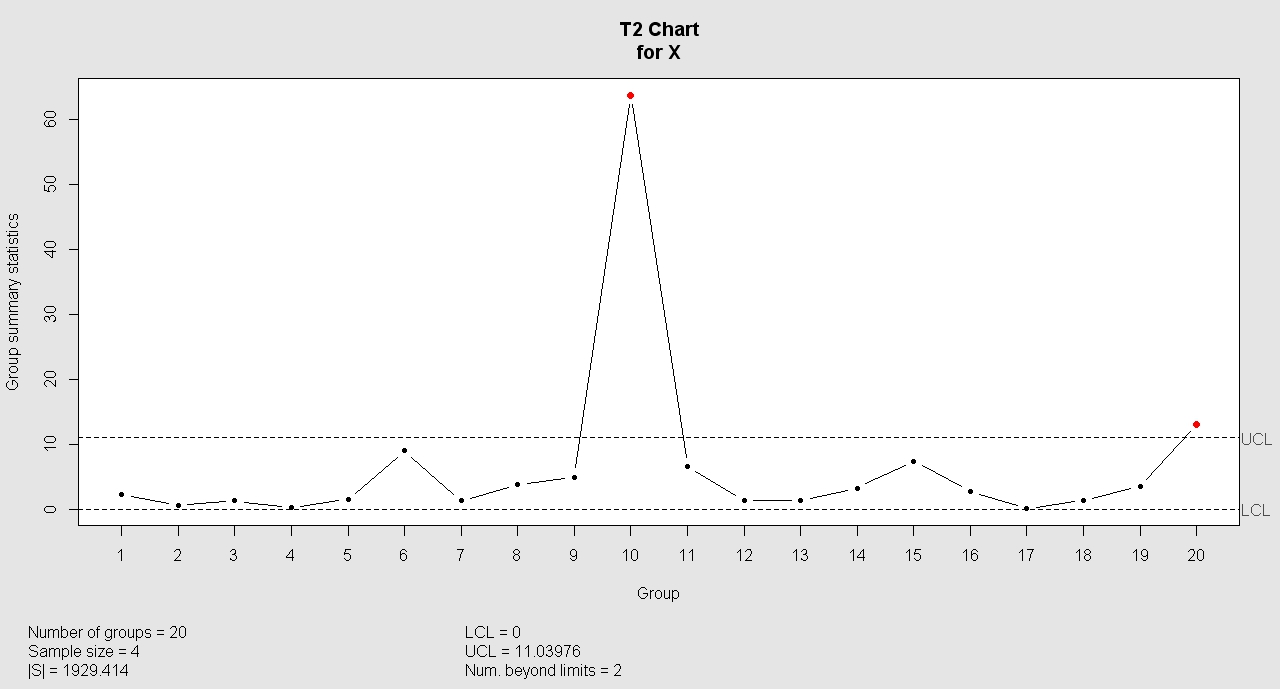
\includegraphics[width=0.9\linewidth]{./mqccplot1}
\caption{}
\label{fig:mqccplot1}
\end{figure}
\newpage
\begin{verbatim}
Call:
mqcc(data = X, type = "T2")

T2 chart for X 

Summary of group statistics:
   Min. 1st Qu.  Median    Mean 3rd Qu.    Max. 
 0.1243  1.3250  2.5030  6.4700  5.3490 63.7600 

Number of variables:  2
Number of groups:  20
Group sample size:  4

Center: 
     X1      X2 
60.3750 18.4875 

Covariance matrix:
         X1        X2
X1 222.0333 103.11667
X2 103.1167  56.57917
|S|:  1929.414 

Control limits:
 LCL      UCL
   0 11.03976

\end{verbatim}
%------------------------------------------- %
\section{The \textbf{qcc} R package - Other Types of Graph}


\subsection{Operating Characteristic (OC) Curves}
\begin{itemize}
\item A common supplementary plot to standard quality control charts is the so-called operating characteristic or OC curve (see example below). One question that comes to mind when using standard variable or attribute charts is how sensitive is the current quality control procedure? Put in more specific terms, how likely is it that you will not find a sample (e.g., mean in an X-bar chart) outside the control limits (i.e., accept the production process as "in control"), when, in fact, it has shifted by a certain amount? 

\item This probability is usually referred to as the  (beta) error probability, that is, the probability of erroneously accepting a process (mean, mean proportion, mean rate defectives, etc.) as being "in control." 

\item Note that operating characteristic curves pertain to the false-acceptance probability using the sample-outside-of- control-limits criterion only, and not the runs tests described earlier.


\item Operating characteristic curves are extremely useful for exploring the power of our quality control procedure. The actual decision concerning sample sizes should depend not only on the cost of implementing the plan (e.g., cost per item sampled), but also on the costs resulting from not detecting quality problems. The OC curve allows the engineer to estimate the probabilities of not detecting shifts of certain sizes in the production quality.
\end{itemize}






\newpage
\subsubsection{pistonrings Data}
\begin{framed}
\begin{verbatim}
data(pistonrings); attach(pistonrings);

diameter <- qcc.groups(diameter, sample)
beta <- oc.curves.xbar(qcc(diameter, type="xbar", nsigmas=3, plot=FALSE))
print(round(beta, digits=4))

# or to identify points on the plot use
## Not run: oc.curves.xbar(qcc(diameter, 
    type="xbar", nsigmas=3, plot=FALSE), identify=TRUE)

detach(pistonrings)
\end{verbatim}
\end{framed}


\newpage
\subsubsection{orangejuice Data}
\begin{framed}
\begin{verbatim}
data(orangejuice)
attach(orangejuice)
beta <- oc.curves(qcc(D[trial], sizes=size[trial], type="p", plot=FALSE))
print(round(beta, digits=4))
# or to identify points on the plot use
## Not run: oc.curves(qcc(D[trial], sizes=size[trial], type="p", plot=FALSE), identify=TRUE)
detach(orangejuice)
\end{verbatim}
\end{framed}
\newpage
\subsubsection{circuit Data}
\begin{framed}
\begin{verbatim}
data(circuit)
attach(circuit)
q <- qcc(x[trial], sizes=size[trial], type="c", plot=FALSE)
beta <- oc.curves(q)
print(round(beta, digits=4))
# or to identify points on the plot use
## Not run: oc.curves(qcc(x[trial], sizes=size[trial], type="c", plot=FALSE), identify=TRUE)
detach(circuit)
\end{verbatim}
\end{framed}
\newpage
\subsection{Moving Average (MA) Chart}
To return to the piston ring example, suppose we are mostly interested in detecting small trends across successive sample means. For example, we may be particularly concerned about machine wear, leading to a slow but constant deterioration of quality (i.e., deviation from specification). The CUSUM chart described above is one way to monitor such trends, and to detect small permanent shifts in the process average. 

Another way is to use some weighting scheme that summarizes the means of several successive samples; moving such a weighted mean across the samples will produce a moving average chart (as shown in the following graph).



\subsection{Exponentially-weighted MA (EWMA) Chart}
The idea of moving averages of successive (adjacent) samples can be generalized. In principle, in order to detect a trend we need to weight successive samples to form a moving average; however, instead of a simple arithmetic moving average, we could compute a geometric moving average (this chart (see graph below) is also called Geometric Moving Average chart, see Montgomery, 1985, 1991).
%-------------------------------------------------- %
\newpage
\subsubsection{Grouped Data}
\begin{framed}
\begin{verbatim}

data(pistonrings)
attach(pistonrings)
diameter <- qcc.groups(diameter, sample)
q <- ewma(diameter[1:25,], lambda=0.2, nsigmas=3)
summary(q)

q <- ewma(diameter[1:25,], lambda=0.2, nsigmas=2.7,
newdata=diameter[26:40,], plot = FALSE)
summary(q)

plot(q)
\end{verbatim}
\end{framed}

\begin{figure}[h!]
\centering
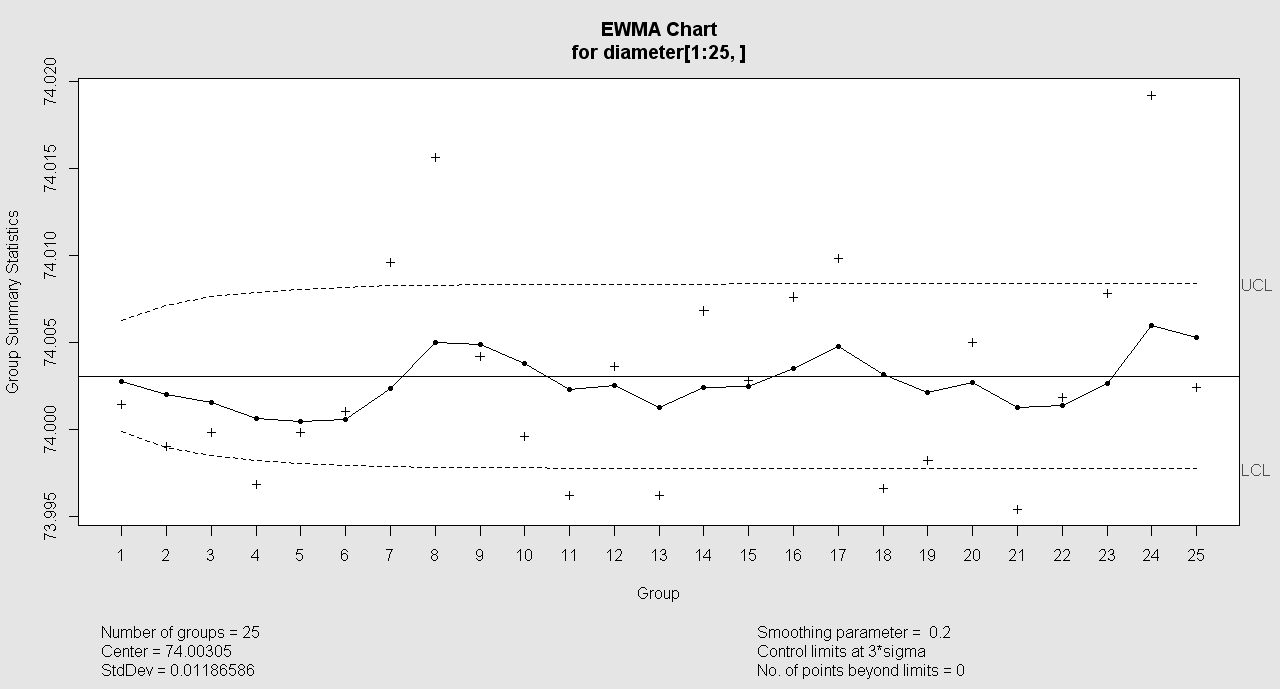
\includegraphics[width=0.6\linewidth]{./qccEWMA1}
\caption{}
\label{fig:qccEWMA1}
\end{figure}
\begin{figure}[h!]
\centering
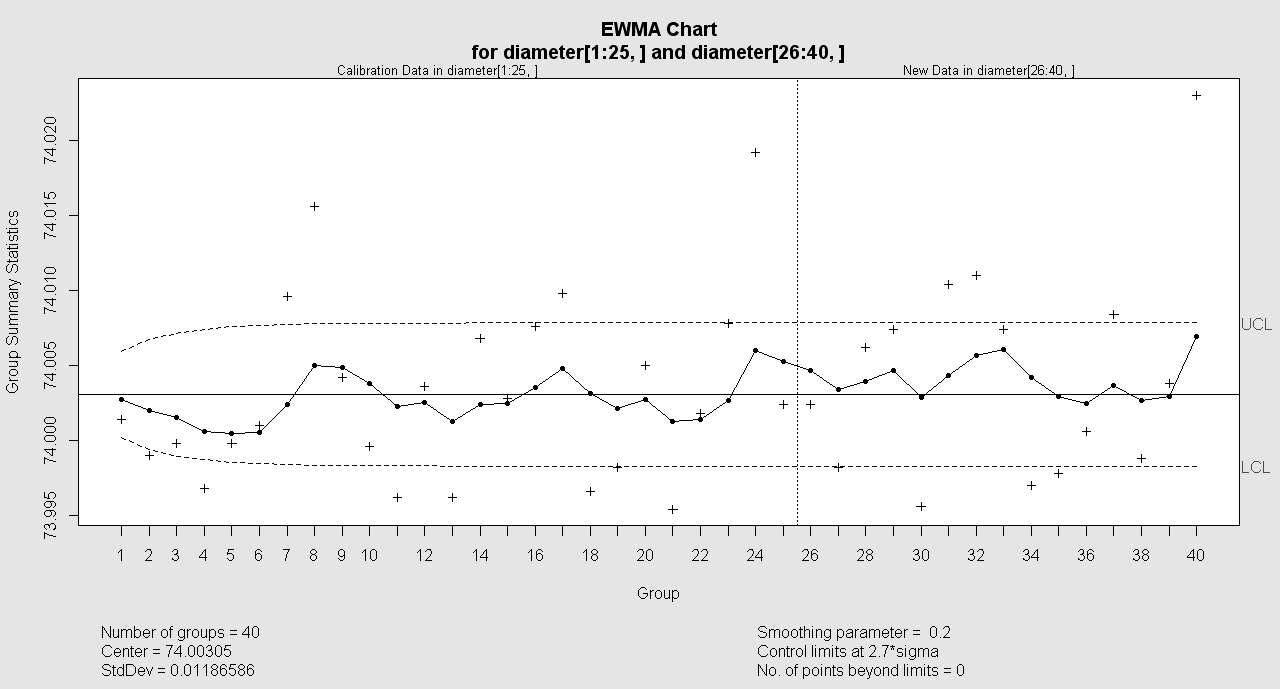
\includegraphics[width=0.6\linewidth]{./qccEWMA2}
\caption{}
\label{fig:qccEWMA2}
\end{figure}
\begin{verbatim}
> summary(q)

Call:
ewma(data = diameter[1:25, ], lambda = 0.2, nsigmas = 2.7, newdata = diameter[26:40,     ], plot = FALSE)

ewma chart for diameter[1:25, ] 

Summary of group statistics:
   Min. 1st Qu.  Median    Mean 3rd Qu.    Max. 
  74.00   74.00   74.00   74.00   74.01   74.02 

Group sample size:  5
Number of groups:  25
Center of group statistics:  74.00305
Standard deviation:  0.01186586 

Summary of group statistics in diameter[26:40, ]:
   Min. 1st Qu.  Median    Mean 3rd Qu.    Max. 
  74.00   74.00   74.00   74.00   74.01   74.02 

Group sample size:  5
Number of groups:  15 

Smoothing parameter: 0.2 
Control limits:
         LCL      UCL
1   74.00018 74.00591
2   73.99938 74.00672
...                  
40  73.99827 74.00782

\end{verbatim}
\newpage
\subsubsection{Individual observations}
\begin{framed}
\begin{verbatim}
x <- c(33.75, 33.05, 34, 33.81, 33.46, 34.02, 33.68, 33.27, 33.49, 33.20,
33.62, 33.00, 33.54, 33.12, 33.84) # viscosity data (Montgomery, pag. 242)
q <- ewma(x, lambda=0.2, nsigmas=2.7)
summary(q)
\end{verbatim}
\end{framed}

\begin{framed}
\begin{verbatim}
x <- 1:50
y <- rnorm(50, sin(x/5), 0.5)
plot(x,y,pch=16,col="blue",font.lab=2)
lines(ewmaSmooth(x,y,lambda=0.1), col="red")
abline(h=mean(y),col="green",lty=2)
title("EWMA Smoother")
\end{verbatim}
\end{framed}
\begin{figure}
\centering
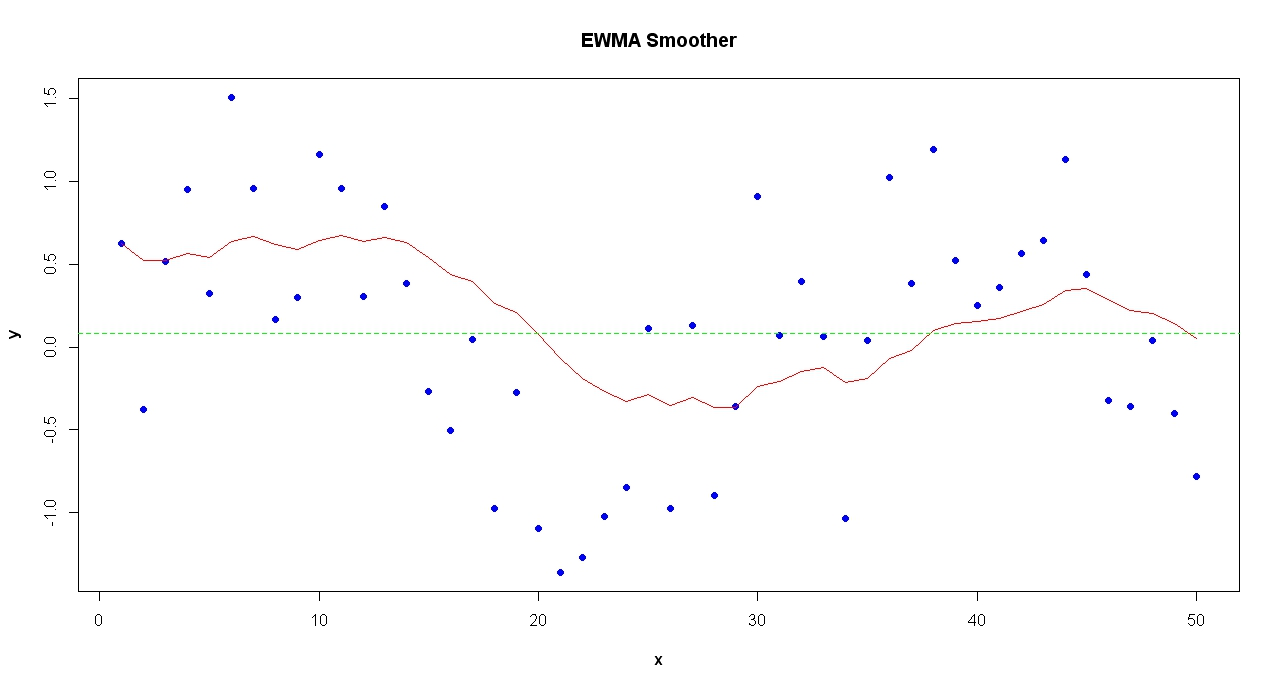
\includegraphics[width=0.7\linewidth]{./qccEWMAsmoother}
\caption{}
\label{fig:qccEWMAsmoother}
\end{figure}
%--------------------------------------------------------------- %
\newpage
\subsection{CUSUM charts}
\begin{itemize}
\item CUSUM charts, while not as intuitive and simple to operate as Shewhart charts, have been shown to be more efficient in detecting small shifts in the mean of a process. \item In particular, analyzing ARL's for CUSUM control charts shows that they are better than Shewhart control charts when it is desired to detect shifts in the mean that are 2 sigma or less.
\end{itemize}

\subsection{Example}
% http://www.itl.nist.gov/div898/handbook/pmc/section3/pmc323.htm

\begin{itemize}
\item The 20 data points are each the average of samples of size 4 taken from a process that has an estimated mean of 325.
\end{itemize}
\begin{framed}
\begin{verbatim}
324.925, 324.675, 324.725, 324.350, 325.350, 325.225, 324.125,
324.525, 325.225, 324.600, 324.625, 325.150, 328.325, 327.250,
327.825, 328.500, 326.675, 327.775, 326.875, 328.350
\end{verbatim}
\end{framed}
%-------------------------------------------------------------- %
\newpage
\subsection{Individual/Moving-Range chart}
% http://en.wikipedia.org/wiki/Shewhart_individuals_control_chart
\begin{itemize}
\item The individual/moving-range chart is a type of control chart used to monitor variables data from a business or industrial process for which it is impractical to use rational subgroups.

\item The chart is necessary in the following situations:
\begin{itemize}
\item[$\ast$] Where automation allows inspection of each unit, so rational subgrouping has less benefit.
\item[$\ast$]Where production is slow so that waiting for enough samples to make a rational subgroup unacceptably delays monitoring
\item[$\ast$] For processes that produce homogeneous batches (e.g., chemical) where repeat measurements vary primarily because of measurement error
\end{itemize}
\item The "chart" actually consists of a pair of charts: one, the individuals chart, displays the individual measured values; the other, the moving range chart, displays the difference from one point to the next. 
\item As with other control charts, these two charts enable the user to monitor a process for shifts in the process that alter the mean or variance of the measured statistic.
\end{itemize}
\newpage
\section{Process Capability}
Process capability is the measure of process performance. Capability refers to the ability of a process to make parts that are well within engineering specifications. A capability study is done to answer the questions, \textit{``Does the process need to be improved?"} and  \textit{``How much does the process need to be improved?"}

To define the study of process capability from another perspective, a capability study is a technique for analyzing the random variability found in a production process. In every manufacturing process there is variability. This variability may be large or small, but it is always present. It can be divided into two types:

\begin{itemize}
\item Variability due to common (random) causes
\item Variability due to assignable (special) causes
\end{itemize}
%----------------------------------------------------------------------------------------------%
The first type of variability can be expected to occur naturally within a process. It is attributed to common causes that behave like a constant system of chances. These chances form a unique and describable distribution. This variability can never be completely eliminated from a process. Variability due to assignable causes, on the other hand, refers to the variation that can be linked to specific or special causes. If these causes, or factors, are modified or controlled properly, the process variability associated with them can be eliminated. Assignable causes cannot be described by a single distribution.
%----------------------------------------------------------------------------------------------%
\newpage
\subsection{Capability Study} 
A capability study measures the performance potential of a process when no assignable causes are present (when it is in statistical control). Since the inherent variability of the process can be described by a unique distribution, usually a normal distribution, capability can be evaluated by utilizing this distribution’s properties. Simply put, capability is expressed as the proportion of in-specification process output to total process input.

Capability calculations allow predictions to be made regarding quality, enabling manufacturers to take a preventive approach to defects. This statistical approach contrasts to the traditional approach to manufacturing, which is a two-step process: production personnel make the product, and quality control personnel inspect and eliminate those products that do not meet specifications. This is wasteful and expensive, since it allows time and materials to be invested in products that are not always usable. It is also unreliable, since even 100\% inspection would fail to catch all defective products.
%----------------------------------------------------------------------------------------------%
Control Limits are Not an Indication of Capability

Those new to SPC often believe they don’t need capability indices. They think they can compare the control limits to the specification limits instead. This is not true, because control limits look at the distribution of averages and capability indices look at the distribution of individuals. The distribution of individuals will always spread out further than the distribution of averages (see figure below). 
%--------------------------------------------------------------------------------------------------%
\newpage
\subsection{What is Process Capability?}

Distribution of averages compared to distribution of individuals, for the same sample data. Control limits (based on averages) would probably be inside specification limits, even though many parts are out of specification. This shows why you should not compare control limits to specification limits.

Therefore, the control limits are often within the specification limits, but the $\pm 3$ Sigma distribution of parts is not.  Subgroup averages follow more closely a normal distribution. This is why we can create control charts for processes that are not normally distributed. But averages cannot be used for capability calculations, because capability concerns itself with individual parts, or samples from a process. After all, parts, not averages, get shipped.

\subsection{Capability Indices}

\begin{description}
\item[Capability] — The uniformity of product which a process is capable of producing. Can be expressed numerically using CP, CR, CpK, and Zmax/3 when the data is normally distributed.

\item[CP] — For process capability studies: CP is a capability index defined by the formula. CP shows the process capability potential but does not consider how centered the process is. CP may range in value from 0 to infinity, with a large value indicating greater potential capability. A value of 1.33 or greater is usually desired.

\item[CR] — For process capability studies: the inverse of CP, CR can range from 0 to infinity in value, with a smaller value indicating a more capable process.

\item[CpK] — For process capability studies: an index combining CP and K to indicate whether the process will produce units within the tolerance limits. CpK has a value equal to CP if the process is centered on the nominal; if CpK is negative, the process mean is outside the specification limits; if CpK is between 0 and 1, then some of the 6 sigma spread falls outside the tolerance limits. If CpK is larger than 1, the 6 sigma spread is completely within the tolerance limits. A value of 1.33 or greater is usually desired.
\end{description}
%---------------------------------------------------------------------------------------------------%
\newpage
\subsection{Interpreting Capability Indices}
\begin{itemize}
\item The greater the CpK value, the better. A CpK greater than 1.0 means that the $6\sigma  (\pm 3\sigma)$ spread of the data falls completely within the specification limits. A CpK of 1.0 means that one end of the $6\sigma$ spread falls on a specification limit. A CpK between 0 and 1 means that part of the $6\sigma$  spread falls outside the specification limits. A negative CpK indicates that the mean of the data is not between the specification limits.

\item Since a CpK of 1.0 indicates that 99.73\% of the parts produced are within specification limits, in this process it is likely that only about 3 out of 1,000 need to be scrapped or rejected. Why bother to improve the process beyond this point, since it will produce no reduction in scrap or reject costs? Improvement beyond just meeting specification may greatly improve product performance, cut warranty costs, or avoid assembly problems.

\item
Many companies are demanding CpK indexes of 1.33 or 2.0 of their suppliers’ products. A CpK of 1.33 means that the difference between the mean and specification limit is $4\sigma$  (since 1.33 is 4/3). With a CpK of 1.33, 99.994\% of the product is within specification. Similarly a CpK of 2.0 is $6\sigma$  between the mean and specification limit (since 2.0 is 6/3). 
\item 
This improvement from 1.33 to 2.0 or better is sometimes justified to produce more product near the optimal target. Depending on the process or part, this may improve product performance, product life, customer satisfaction, or reduce warranty costs or assembly problems.
\item
Continually higher CpK indexes for every part or process is not the goal, since that is almost never economically justifiable. A cost/benefit analysis that includes customer satisfaction and other true costs of quality is recommended to determine which processes should be improved and how much improvement is economically attractive.
\end{itemize}

\subsection{Process Capability Analysis}
{
\large

\begin{itemize}
\item Process capability compares the output of an in-control process to the specification limits by using capability indices.
\item The comparison is made by forming the ratio of the spread between the process specifications (the specification "width") to the spread of the process values, as measured by 6 process standard deviation units (the process "width").
\end{itemize}
\newpage
\subsection{Intepreting Process Capability Indices}
\begin{itemize}
\item \textbf{CP}\\
Historically, this is one of the first capability indexes used. The "natural tolerance" of the process is computed as 6s . The index simply makes a direct comparison of the process natural tolerance to the engineering requirements. Assuming the process distribution is normal and the process average is exactly centered between the engineering requirements, a CP index of 1 would give a "capable process." However, to allow a bit of room for process drift, the generally accepted minimum value for CP is 1.33. In general, the larger CP is, the better. The CP index has two major shortcomings. First, it cannot be used unless there are both upper and lower specifications. Second, it does not account for process centering. If the process average is not exactly centered relative to the engineering requirements, the CP index will give misleading results. In recent years, the CP index has largely been replaced by CPK (see below).

\item \textbf{CR}\\
The CR index is algebraically equivalent to the CP index. The index simply makes a direct comparison of the process to the engineering requirements. Assuming the process distribution is normal and the process average is exactly centered between the engineering requirements, a CR index of 100\% would give a "capable process." However, to allow a bit of room for process drift, the generally accepted maximum value for CR is 75\%. In general, the smaller CR is, the better. The CR index suffers from the same shortcomings as the CP index.

\item\textbf{ ZU}\\
The ZU index measures the process location (central tendency) relative to its standard deviation and the upper requirement. If the distribution is normal, the value of ZU can be used to determine the percentage above the upper requirement by using Table 4 in the appendix of The Complete Guide to the CQM. The method is the same as described in Chapter III.B using the Z statistic, simply use ZU instead of using Z. In general, the bigger ZU is, the better. A value of at least +3 is required to assure that 0.1\% or less defective will be produced. A value of +4 is generally desired to allow some room for process drift.

\item \textbf{ZL}\\
The ZL index measures the process location relative to its standard deviation and the lower requirement. If the distribution is normal, the value of ZL can be used to determine the percentage above the upper requirement by using Table 4 in the appendix of The Complete Guide to the CQM. The method is the same as described in III.B [of The Complete Guide to the CQM] using the Z transformation, except that you use -ZL instead of using Z. In general, the bigger ZL is, the better. A value of at least +3 is required to assure that 0.1\% or less defective will be produced. A value of +4 is generally desired to allow some room for process drift.

\item \textbf{ZMIN}\\
The value of ZMIN is simply the smaller of the ZL or the ZU values. It is used in computing CPK.

\item\textbf{ CPK}\\
The value of CPK is simply ZMIN divided by 3. Since the smallest value represents the nearest specification, the value of CPK tells you if the process is truly capable of meeting requirements. A CPK of at least +1 is required, and +1.33 is preferred. Note that CPK is closely related to CP, and that the difference between CPK and CP represents the potential gain to be had from centering the process.

\item\textbf{ CPM}\\
A CPM of at least 1 is required, and 1.33 is preferred. CPM is closely related to CP. The difference represents the potential gain to be obtained by moving the process mean closer to the target. Unlike CPK, the target need not be the center of the specification range.
\end{itemize}
\newpage
\subsubsection{Capability Index Example}
\begin{itemize}
\item For a certain process the USL=20 and the LSL=8. The observed process average, $\bar{x}$$\geq$16, and the standard deviation, s=2. 
\item 
From this we obtain
\[C^p=\frac{USL-LSL}{6s}= \frac{20−8}{6(2)}=1.0.\]
\item This means that the process is capable as long as it is located at the midpoint, m=(USL+LSL)/2=14.
\item But it doesn't, since $\bar{x}\geq16$. 
\item The $\hat{k}$ factor is found by
\[\hat{k}=\frac{|m−\bar{x}|(USL−LSL)}/2=26=0.3333\]
and
\[C^pk=C^p(1−\hat{k})=0.6667.\]
\item We would like to have $C^pk$ at least 1.0, so this is not a good process. If possible, reduce the variability or/and center the process. \item We can compute the $C^pu$ and $C^pu$ using
\[C^pu=USL−\bar{x}3s=20-163(2)=0.666\]
and
\[C^pl=\bar{x}-LSL3s=16−83(2)=1.3333.\]
\item From this we see that the $C^pu$, which is the smallest of the above indices, is 0.6667. 
\item Note that the formula $C^pk=C^p(1−\hat{k})$ is the algebraic equivalent of the $min(C^pu,C^pl)$ definition.
\end{itemize}
}
%------------------------------------------------------ % 
\newpage






%------------------------------------------------------- %
\newpage
\section{Six Sigma R Package}
\begin{figure}[h!]
\centering

\includegraphics[width=0.4\linewidth]{./sixsigmalogo}
\caption{}
\label{fig:sixsigmalogo}
\end{figure}

\subsection{DMAIC Process}
\begin{itemize}
\item DMAIC (an abbreviation for Define, Measure, Analyze, Improve and Control) refers to a data-driven improvement cycle used for improving, optimizing and stabilizing business processes and designs.
\item  The DMAIC improvement cycle is the core tool used to drive Six Sigma projects. 
\item However, DMAIC is not exclusive to Six Sigma and can be used as the framework for other improvement applications.
\end{itemize}
\subsection{Data Set - \texttt{ss.data.ca} }
This data set is the volume measured in 20 bottles for a filling process in a winery
\begin{framed}
\begin{verbatim}
ss.data.ca
\end{verbatim}
\end{framed}

\begin{verbatim}
> ss.data.ca
   Volume
1  755.81
2  750.54
........
........
19 750.26
20 751.29
\end{verbatim}
\begin{figure}[h!]
\centering
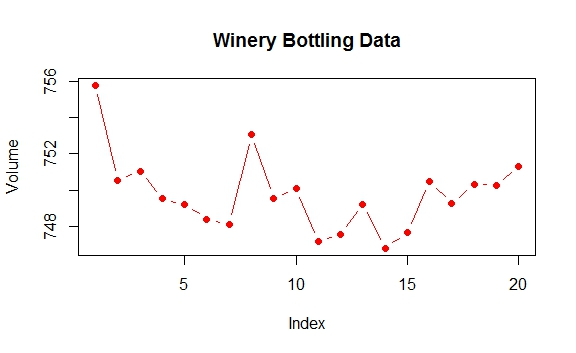
\includegraphics[width=0.9\linewidth]{./Winery}
\caption{}
\label{fig:Winery}
\end{figure}

%----------------------------------------------------------------------------------------------%
\newpage
\subsection{\texttt{ss.ca.z} Capability Indices}

Compute the Capability Indices of a process, Z (Sigma Score), $C_p$ and $C_{pk}$.
\begin{verbatim}
> ss.ca.cp(ss.data.ca$Volume,740, 760)
[1] 1.584136
> ss.ca.cpk(ss.data.ca$Volume,740, 760)
[1] 1.546513
> ss.ca.z(ss.data.ca$Volume,740,760)
[1] 3.139539
\end{verbatim}



\newpage
\subsection{Constructing Process Maps}
\begin{framed}
\begin{verbatim}
inputs.overall<-c("operators", "tools", "raw material", "facilities")
outputs.overall<-c("helicopter")
steps<-c("INSPECTION", "ASSEMBLY", "TEST", "LABELING")
\end{verbatim}
\end{framed}

\begin{framed}
\begin{verbatim}
#Inputs of process "i" are inputs of process "i+1"
input.output<-vector(mode="list",length=length(steps))
input.output[1]<-list(c("sheets", "..."))
input.output[2]<-list(c("sheets"))
input.output[3]<-list(c("helicopter"))
input.output[4]<-list(c("helicopter"))
\end{verbatim}
\end{framed}
Parameters of each process
\begin{framed}
\begin{verbatim}

x.parameters<-vector(mode="list",length=length(steps))

x.parameters[1]<-list(c(list(c("width", "NC")),list(c("operator", "C")),
                        list(c("Measure pattern", "P")), list(c("discard", "P"))))
x.parameters[2]<-list(c(list(c("operator", "C")),list(c("cut", "P")),
                        list(c("fix", "P")), list(c("rotor.width", "C")),
                        list(c("rotor.length",                                                                                "C")), 
                                                                                list(c("paperclip", "C")), list(c("tape", "C"))))
x.parameters[3]<-list(c(list(c("operator", "C")),
list(c("throw", "P")),
                        list(c("discard", "P")), 
                        list(c("environment", "N"))))
x.parameters[4]<-list(c(list(c("operator", "C")),
list(c("label", "P"))))
x.parameters

\end{verbatim}
\end{framed}

\begin{framed}
\begin{verbatim}
#Features of each process
y.features<-vector(mode="list",length=length(steps))
y.features[1]<-list(c(list(c("ok", "Cr"))))
y.features[2]<-list(c(list(c("weight", "Cr"))))
y.features[3]<-list(c(list(c("time", "Cr"))))
y.features[4]<-list(c(list(c("label", "Cr"))))
y.features
ss.pMap(steps, inputs.overall, outputs.overall,
        input.output, x.parameters, y.features,
        sub="Paper Helicopter Project")
\end{verbatim}
\end{framed}
\begin{figure}[h!]
\centering
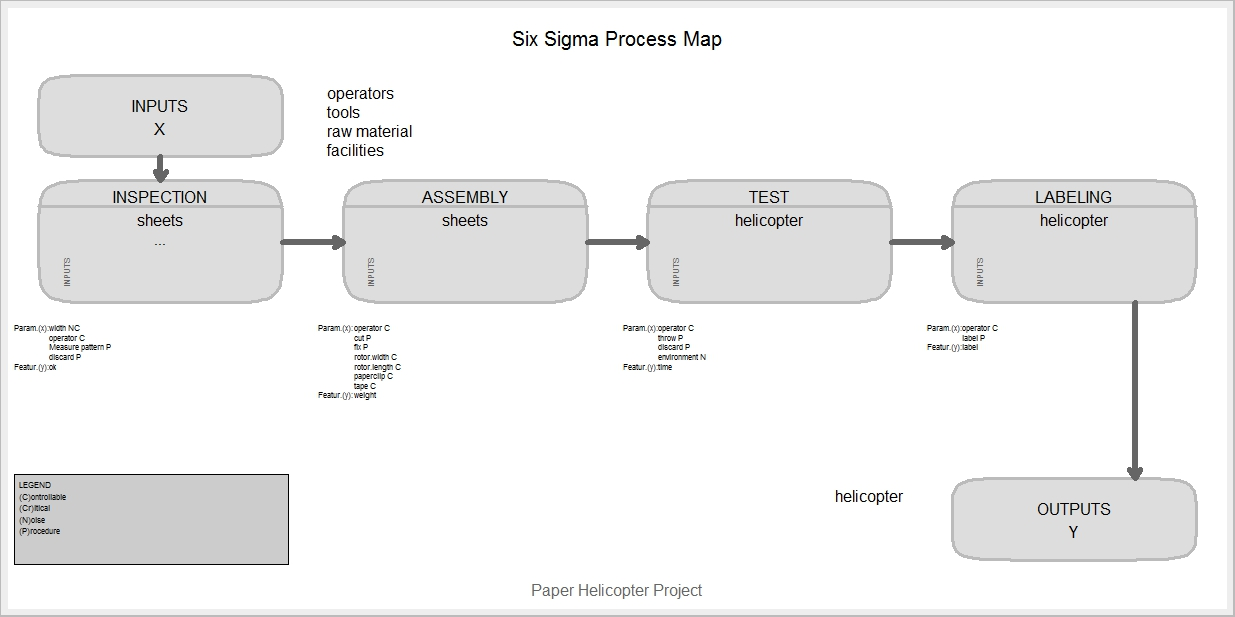
\includegraphics[width=0.9\linewidth]{./SixSigmaProcessMap}
\caption{}
\label{fig:SixSigmaProcessMap}
\end{figure}
%--------------------------------------------------- %
\newpage
\subsection{Loss Fucntion Aanalysis}
The Taguchi Loss Function is graphical depiction of loss developed by the Japanese business statistician Genichi Taguchi to describe a phenomenon affecting the value of products produced by a company. Praised by Dr. W. Edwards Deming (the business guru of the 1980s American quality movement),[1] it made clear the concept that quality does not suddenly plummet when, for instance, a machinist exceeds a rigid blueprint tolerance. Instead "loss" in value progressively increases as variation increases from the intended condition. This was considered a breakthrough in describing quality, and helped fuel the continuous improvement movement that since has become known as lean manufacturing.

\begin{figure}[h!]
\centering
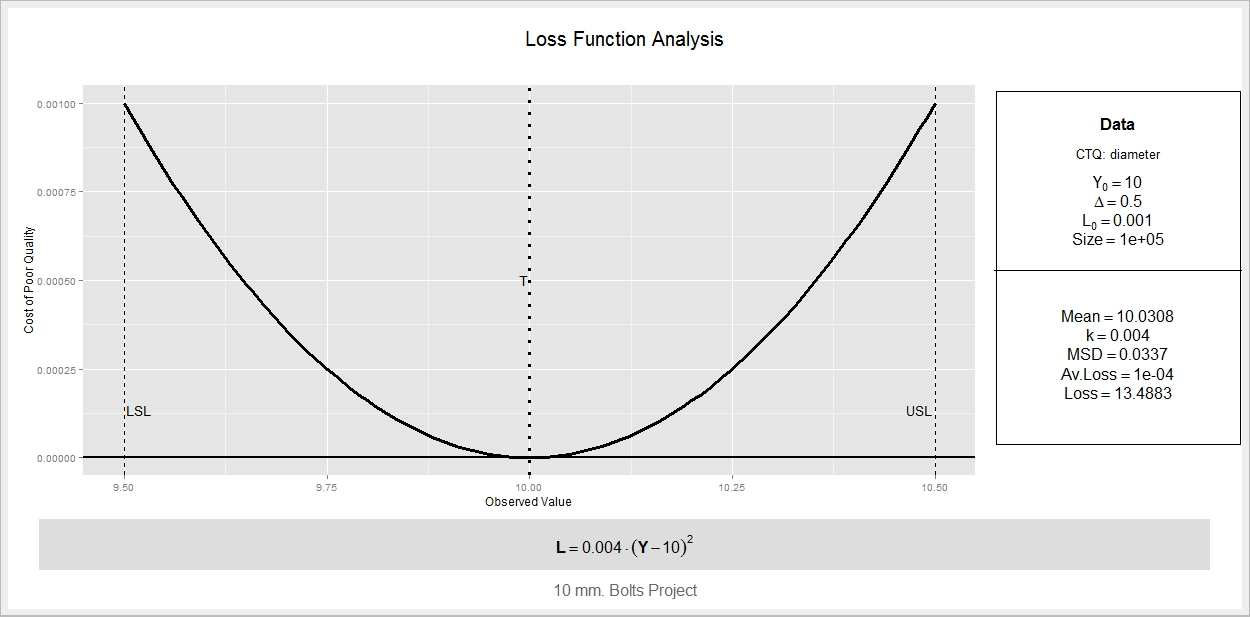
\includegraphics[width=0.7\linewidth]{./LossFunctionAnalysis}
\caption{}
\label{fig:LossFunctionAnalysis}
\end{figure}
%------------------------------------------------------- %
\newpage
\section{Other R Packages}

\begin{enumerate}
\item mpci
\item mspc
\item qualityTools
\item spc
\item SixSigma with R (Emilio Cano)
\end{enumerate}

\tableofcontents
%------------------------------------------------------ %

\newpage
%----------------------------------------------------------------------------------------------%


\newpage
\subsection{ \texttt{spc}: Statistical Process Control }

% Collection of Some Useful Functions

\begin{itemize}
\item Evaluation of control charts by means of the zero-state, steady-state ARL (Average Run Length) and RL quantiles. 

\item Setting up control charts for given in-control ARL. 

\item The control charts under consideration are one- and two-sided EWMA, CUSUM, and Shiryaev-Roberts schemes for monitoring the mean of normally distributed independent data. 

\item
ARL calculation of the same set of schemes under drift are added. 

\item Other charts and parameters are in preparation. 

\item Further SPC areas will be covered as well (sampling plans, capability indices ...)
\end{itemize}

%---------------------------------------------------------------------------------------------%

R package spc provides

\begin{verbatim}
xcusum.ad steady-state ARLs of CUSUM charts
xcusum.arl (zero-state) ARLs of CUSUM charts
xcusum.crit decision intervals of CUSUM charts
xewma.ad steady-state ARLs of EWMA charts
xewma.arl (zero-state) ARLs of EWMA charts
xewma.crit critical values of EWMA charts
\end{verbatim}




\end{document}
